\documentclass{article}
\usepackage[utf8]{inputenc}

\title{Chem-131C-Lec13}

\author{swflynn }
\date{May 2017}

\usepackage{natbib}
\usepackage{graphicx}
\usepackage{braket}
\usepackage{amsmath}
\usepackage[margin=0.7in]{geometry}
\usepackage{subfigure}
\usepackage{url}
\usepackage{float}

\begin{document}

\maketitle

\section*{Lecture 13; 5/1/17}
Note the midterm will be next Friday, May 12 during lecture. 
A single note card will be allowed in during the exam, more details will be given before the exam. 

\subsection*{Heat Capacity and Entropy}
Consider a metal block you just took out of the oven, with a heat capacity C and a temperature T$_H$. 
Throw the block into the ocean which also has a heat capacity C$_1$ at a temperature T$_C$. 
What is the minimum entropy change of the universe? 

To solve this question we note that the block is at a higher temperature than the ocean, and therefore heat will transfer from the block to the ocean. 
We next assume that the ocean is so large compared to the block that the small amount of heat dismissed by the block cannot actually change the temperature of the ocean (remember temperature is an average over all the atoms... to change that is not easy).
This means the block will go from T$_H \rightarrow T_C$. 
The change in the temperature of the block (which is due to the heat flowing out of the block into the ocean) can be calculated as 
\begin{equation}
   Q = \int_{T_H}^{T_C}CdT = C \int_{T_H}^{T_C}dT = C(T_H-T_C)
\end{equation}
The entropy of the universe can be thought of as the entropy of the block plus the entropy of the ocean, the entropy of the block decreases because the block is losing heat, but the ocean will increase. 
\begin{equation}
   \begin{split}
       S &\equiv \frac{q_{rev}}{T}, \qquad \Delta S_{univ} = \Delta S + \Delta S_{surr} \\
       \Delta S_{univ} &= \left(\int_{T_H}^{T_C} C \frac{dT}{T}\right) + \frac{q}{T_C} \\
       &= C\ln\left(\frac{T_C}{T_H}\right) + \frac{C(T_H-T_C)}{T_C} = C\ln\left(\frac{T_C}{T_H}\right) + C\left(\frac{T_H}{T_C}- 1\right)
   \end{split}
\end{equation}
We now expect this to be greater than 0, we could just run some numbers to show this numerically. 
But consider x$\equiv \frac{T_H}{T_C}$, we are therefore asking is x-1 $\geq$ ln x. 
\begin{equation}
\begin{split}
    -C\ln\left(\frac{T_H}{T_C}\right) + C\left(\frac{T_H}{T_C}- 1\right) \geq 0\\
      -C\ln x + C\left(x- 1\right) \geq 0\\
\end{split}
\end{equation}
When we plot these two function it becomes apparent that the entropy of the universe must be $\geq$ 0.
\begin{figure}[H]
    \centering
    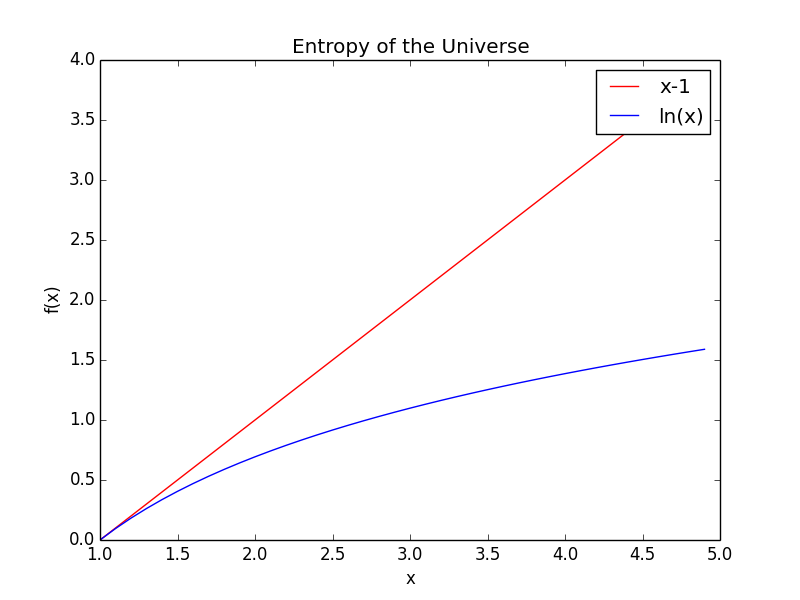
\includegraphics[width=15cm]{myfig.png}
    \caption{Entropy Analysis. We see that the entropy of the universe must increase for all temperature ratios.}
    \label{fig:entropy}
\end{figure}

\subsection*{Energy of a Bike Pump}
Consider a new problem, we are pumping air into a bicycle tire. 
We will assume the pumping is done adiabatically, but the pump will start to feel warmer due to the work it is doing. 
So we sit there and we push down on the pump to put air in the tire, and then we pull up on the pump to reset and push again.
In the language of thermodynamics we are doing a series of adiabatic, irreversible (assume we push with constant pressure) compression's and expansions. 

Intuitively we know that the external pressure we use for the compression must be larger than that of the expansion.
Because the process is $\approx$ adiabatic, U = w
If we consider 1 cycle (1 compression and then 1 expansion), we know that U
\begin{equation}
\Delta U_{cycle} = \Delta U_c + \Delta U_e = w_c + w_e
\end{equation}
The work for this irreversible process is simply -P$_{ext}\Delta V$ therefore 
\begin{equation}
\Delta U_{cycle} = -P_{ext,c}(V_f-V_i) + -P_{ext,e}(V_i-V_f)
\end{equation}
If we were interested in the temperature we can make an equality through the internal energy (heat capacity is found through the total differential of U(T,n).
\begin{equation}
\begin{split}
U(T) &\rightarrow \frac{d}{dT}U dT \equiv C \implies \\
\Delta U &= nC\Delta T
\end{split}
\end{equation}

\subsection*{Flipping Coins}
Let's change gears and do a statistical mechanics question now. 
Consider 2 coins, let's consider one coin to be fair (a=0.5) and the other to be bias (a=0.75), for the probability of getting a heads. 

\subsubsection*{What is the probability of getting 1 head and 1 tail?}

From Lecture 9, we discussed the PGF for a fair coin as 
\begin{equation}
F_f(x) = \frac{1}{2}+\frac{1}{2}x
\end{equation}
We can simply recall the definition for the PGF and write the equivalent statement for the unfair coin.
\begin{equation}
F_u(x) = \frac{3}{4}+\frac{1}{4}x
\end{equation}
We can also enumerate the scenario, there are 4 options, assume the first coordinate is the fair coin and the second is the bias coin.
[HH,HT,TH,TT] = [(.5)(.75), (.5)(.25), (.5)(.75), (.5)(.25)]
Combining the cases we see that the 2 coins being flipped have pprobabilities of $\frac{3}{8}$ + $\frac{1}{2}$ and $\frac{1}{8}$x$^2$ (HH,HT,TT respecively).

\subsubsection*{What is the Gibbs Entropy for the System?}
We were introduced to the Gibbs Entropy on Assigned Problem Set 2.
\begin{equation}
\frac{S}{k}= -\sum_jP_j\ln(P_j)
 \end{equation}
We simply need to plug in and solve for the 3 different states in the system (assume number of heads defines our system).
\begin{equation}
    \begin{split}
    \frac{S}{k}^{bias} &= -\frac{3}{8}\ln \left(\frac{3}{8}\right) + -\frac{1}{2}\ln\left(\frac{1}{2}\right) + -\frac{1}{8}\ln\left(\frac{1}{8}\right) \\
    \frac{S}{k}^{fair} &= -\frac{1}{4}\ln \left(\frac{1}{4}\right) + -\frac{1}{2}\ln\left(\frac{1}{2}\right) + -\frac{1}{4}\ln\left(\frac{1}{4}\right)
        \end{split}
\end{equation}

\subsection*{Name}
Consider a monoatomic gas (n=1) contained in a fixed volume adiabatic cylinder, with an adjustable piston. 
The system begins in mechanical equilibrium with the outside pressure P$_0$. 
We then add some heat into the system (no heat can leave still), determine the final P, V, $\Delta$U, $\Delta$S, $\Delta$H.

From intuition we know that the temperature of the system must increase if heat can't leave, and the volume will expand until the gas reaches equilibrium with the atmospheric pressure again(P = P$_0$). 
Using our equation of state and the final pressure we write. 
\begin{equation}
    \begin{split}
        PV &= nRT \implies \frac{PV}{T} = \text{constant} \\
        \frac{P_0V_0}{T_0} &= \frac{PV}{T} \text{substitute P=P$_0$} \\
        V &= \frac{V_0T}{T_0}
    \end{split}
\end{equation}
Nothing in this problem suggested it was done reversibly therefore we calculate the work as follows.
\begin{equation}
        w \equiv -\int_{v_0}^V P_{ext}dV = -P_0(V-V_0)
\end{equation}
We now need to solve for the final temperature, we will do this by equating the first law with the ideal gas model.
Because this is an ideal monoatomic gas we can write an equation for the internal energy using the equipartition theorem. 
\begin{equation}
        \begin{split}
           U(T) \rightarrow U &= \frac{3}{2}nRT \implies \Delta U = \frac{3}{2}R\Delta T \\
           \frac{3}{2}R\Delta T &= q + -P_0(V-V_0)\\
           q &= \frac{3}{2}R(T-T_0) + P_0V_0\left(\frac{T}{T_0}-1\right) \\
           T &= T_0\left(  \frac{q+\frac{3}{2}RT_0+P_0V_0}{\frac{3}{2}RT_0+P_0V_0} \right)\\
           V &= V_0\left(  \frac{q+\frac{3}{2}RT_0+P_0V_0}{\frac{3}{2}RT_0+P_0V_0} \right)
        \end{split}
\end{equation}
The last line follows immediately because T and V have a linear relationship (Ideal Gas EOS).

We can now calculate the entropy change of the system using our adiabatic entropy equation
\begin{equation}
\begin{split}
        \Delta S = R\ln\left[ \left(\frac{T}{T_0}\right)^{\frac{3}{2}}\left(\frac{V}{V_0}\right) \right] \\
        \end{split}
\end{equation}
If we simply look at the forms of the T and V we see that they are the same relationship therefore. 
\begin{equation}
    \Delta S = R\ln\left( \frac{Q+\frac{3}{2}RT_0+P_0V_0}{\frac{3}{2}RT_0+P_0V_0} \right)^{\frac{5}{2}}
\end{equation}
Finally we can calculate the enthalpy. 
By Definition (see lecture 7 Supplemental).
\begin{equation}
\begin{split}
    \Delta H = \Delta U + \Delta(PV) \\
    \Delta H = \Delta U + P\Delta(V)\\
    \Delta H = q
    \end{split}
\end{equation}
Here the pressure was pulled out of the differential because it is constant at the beginning/end states, and the last line follows from the first law. 

\end{document}